%! Author = taj
%! Date = 7/22/25

% Preamble
\documentclass[11pt]{article}

% Packages
\usepackage{amsmath}
\usepackage{graphicx}
\usepackage{float}
\usepackage{upgreek}

\title{10. Merjenje specifične toplote snovi}
\author{Taj Šobot}

% Document
\begin{document}
    \maketitle
    \flushleft
    Pri tem eksperimentu smo probali izračunat specifično toploto poljubnih kovin.

    Skica eksperimenta (kalorimetra):
    \begin{figure}[H]
        \centering
        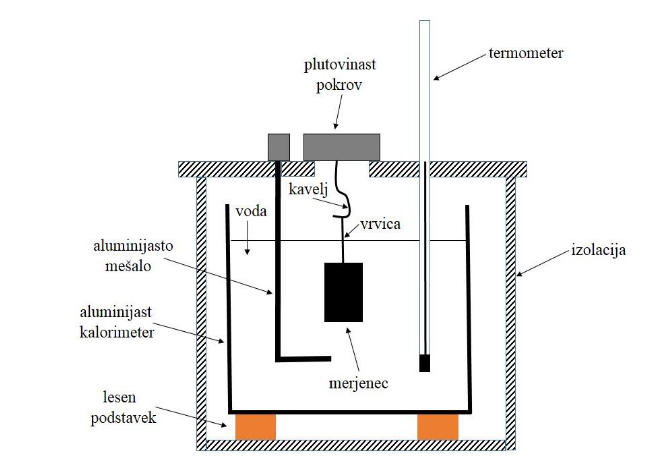
\includegraphics[width=0.9\textwidth]{img}
        \caption{Skica eksperimenta}
        \label{fig:1}
    \end{figure}

    \section{Meritve}

    Mase merjencev:
    \[
        m_{al} = (140 \pm 1)g \, \, m_{cu} = (437 \pm 1) g
    \]
    Masa notranje posode:
    \[
        m_p = (87 \pm 1) g
    \]
    Masa mešala:
    \[
        m_m = (24.1 \pm 1) g
    \]
    Masa vode:
    \[
        m_v = (603 \pm 1)
    \]
    Tempratura vode:
    \[
        T_v = 99.5 ^{\circ}C = (372.5 \pm 0.2) K
    \]
    Ko smo mase premaknili v kalorimeter smo odčitali začetno in končno (ustaljeno) temperaturo:
    \begin{align*}
        Cu: \\
        T_z = (293.7 pm 0.2) K \\
        T_k = (298.4 pm 0.2) K \\
        Al: \\
        T_z = (298.4 pm 0.2) K \\
        T_k = (301.5 pm 0.2) K \\
    \end{align*}

    \section{Rezultati}

    Specifično toploto aluminija lahko izračunamo tako (kalorimeter in mešalna palica sta tudi iz aluminija):
    \[
        c_{al} = \frac{m_v c_v (T^{(k) - T^{(z)}})}{m_k (T_k^{(z)} - T^{(k)}) - m'(T^{(k)} - T^{(z)})} = (816 \pm 8) \frac{J}{kg K}
    \]
    Torej toplotna kapaciteta:
    \[
        C = c_{al m'} = (91 \pm 2) \frac{J}{K}
    \]
    Za Cu pa moramo uporabiti drugo enačbo:
    \begin{align*}
        c_{cu} =  \frac{m_v c_v (T^{(k) - T^{(z)}}) + C(T^{(k) - T^{(z)}})}{m_k (T_k^{(z)} - T^{(k)})} =  (380 \pm 8) \frac{J}{kg K}
    \end{align*}

    Te vrednosti so presenetljivo blizu realnim!

    Vprašanje: izračun specifičnih toplot z Dullong-Petitovo
    enačbo:
    \begin{align*}
        c_{al} = \frac{3 R}{M_{al}} = 924 \frac{J}{kg K} \\
        c_{cu} = \frac{3 R}{M_{cu}} = 392 \frac{J}{kg K} \\
    \end{align*}

\end{document}